
\section{Execution}
\label{sec:exec}
Executing \textit{FloatingSE} requires additional inputs beyond those of
the geometry definition described above in Section \ref{sec:geom}.
Other user inputs for the metocean and loading environment, and the
operational constraints, are required to evaluate the total mass, cost,
and code compliance.  These variables are described below, followed by
the sequence of \textit{FloatingSE} calculations.

\subsection{User Inputs}
The remaining input variables beyond those listed in Section
\ref{sec:geom} describe the metocean environment, the turbine geometry
and loading, as well as loading constraints.  The loading constraints
are more relevant in the context of optimization, so they are described
later in Section \ref{sec:opt}.  The remaining variables are explained
below.

\subsubsection{Load Cases}
The user must specify the metocean conditions that drive the wind and
wave loads upon the floating substructure.  Ideally, multiple metocean
conditions would be used for design optimization.  This includes
standard operating conditions that determine fatigue loads, maximum
allowable operating conditions (e.g. max thrust), maximum survivable
conditions even if the rotor blades are parked, and likely others that
bound a design.  As of this writing, \textit{FloatingSE} only supports
execution and optimization around a single metocean condition and load
case.  Future development will enable optimization against multiple load
cases in a computationally efficient manner.

\subsubsection{Metocean Environment}
The metocean condition is specified by the water and wind environment.
Geographical dependence is chiefly captured by specifying the water
depth.  The wave loading is parameterized by setting the significant
wave height, periodicity, and mean current speed (if any).  Physical
properties of the water, specifically the density and viscosity, are
also captured.  The user may also set the added mass constant used in
Equation \ref{eqn:morison} (Morison's equation).  All of these variables
cumulatively are,

{\footnotesize
  \begin{tabularx}{\linewidth}{ l l X }
    \textbf{Variable} & \textbf{Type} & \textbf{Description \& units} \\
    \texttt{water\_depth} & Float scalar & Distance to sea floor [$m$]\\
    \texttt{hmax}        & Float scalar & Significant wave height [$m$]\\
    \texttt{T}           & Float scalar & Wave period [$s$]\\
    \texttt{cm}          & Float scalar & Added mass coefficient\\
    \texttt{Uc}          & Float scalar & Mean current speed [$m/s$]\\
    \texttt{z0}          & Float scalar & z-coordinate of water line [$m$]\\
    \texttt{water\_density}      & Float scalar & Density of water [$kg/m^3$]\\
    \texttt{base.waveLoads.mu}  & Float scalar & Viscosity of water [$kg/m/s$]\\
  \end{tabularx}
}

Not that the some of these variables, especially the one setting water
viscosity, are awkwardly posed and named.  This is due
to the need for OpenMDAO to have only one independent variable in any
high-level group.  Since \textit{FloatingSE} is intended to be married
with other WISDEM modules in simulation of a full turbine, the design
load cases must be specified at this higher-level group.  Thus,
\textit{FloatingSE} cannot declare independent variables relevant to the
load cases on its own, and must therefore use the variable names as
originally developed in the original modules.

The wind profile is specified by the user with a reference height and
velocity.  From there, wind speeds at other heights are determined using
a shear exponent, for power-law scaling, althrough logarithmic scaling
is available as well.  The physical properties of the air at the turbine
location must also be set.  As with the water-relevant variables, the
comment of awkwardly labeled variables applies.  Cumulatively, all of
the wind-related variables are,

{\footnotesize
  \begin{tabularx}{\linewidth}{ l l X }
    \textbf{Variable} & \textbf{Type} & \textbf{Description \& units} \\
    \texttt{Uref}        & Float scalar & Wind reference speed [$m/s$]\\
    \texttt{zref}        & Float scalar & Wind reference height [$m$]\\
    \texttt{shearExp}    & Float scalar & Shear exponent in wind power law\\
    \texttt{beta}        & Float scalar & Wind beta angle [$deg$]\\
    \texttt{cd\_usr}      & Float scalar & Set to inf or nan to compute by Reynolds number\\
    \texttt{base.windLoads.rho} & Float scalar & Density of air [$kg/m^3$]\\
    \texttt{base.windLoads.mu}  & Float scalar & Viscosity of air [$kg/m/s$]\\
  \end{tabularx}
}


\subsubsection{Turbine Description}
To successfully analyze the entire load path through the substructure,
the user, or other WISDEM modules, must input the geometry and loading of
the wind turbine above the substructure.  The next component after the
substructure in the load path is the tower.  As a long, slender column,
the tower geometry parameterization is similar to that of the
substructure columns,

{\footnotesize
  \begin{tabularx}{\linewidth}{ l l X }
    \textbf{Variable} & \textbf{Type} & \textbf{Description \& units} \\
    \texttt{hub\_height}              & Float scalar & Length from tower base to top (not including freeboard) [$m$]\\
    \texttt{tower\_section\_height}    & Float array ($nSection$) & Length of each tower section [$m$]\\
    \texttt{tower\_outer\_diameter}    & Float array ($nSection+1$) & Diameter at each tower section node (linear lofting between) [$m$]\\
    \texttt{tower\_wall\_thickness}    & Float array ($nSection+1$) & Diameter at each tower section node (linear lofting between) [$m$]\\
    \texttt{tower\_buckling\_length}   & Float scalar & Tower buckling reinforcement spacing [$m$]\\
    \texttt{tower\_outfitting\_factor} & Float scalar & Scaling for unaccounted tower mass in outfitting\\
  \end{tabularx}
}

TODO: REFERENCE TOWERSE and JACKETSE DOCS

At the top of the load path, above the tower, is the rotor nacelle
assembly (RNA).  The RNA includes the blades, hub, shaft(s), gearbox,
generator, nacelle housing, etc.  All of these components are addressed
in WISDEM, but \textit{FloatingSE} only requires aggregate summations of
the mass properties, forces, and moments.  These cumulative variables are,

{\footnotesize
  \begin{tabularx}{\linewidth}{ l l X }
    \textbf{Variable} & \textbf{Type} & \textbf{Description \& units} \\
    \texttt{rna\_mass}   & Float scalar & Mass [$kg$]\\
    \texttt{rna\_I}      & Float array (6) & Moment of intertia (xx,yy,zz,xy,xz,yz) [$kg/m^2$]\\
    \texttt{rna\_cg}     & Float array (3) & Offset of RNA center of mass from tower top (x,y,z) [$m$]\\
    \texttt{rna\_force}  & Float array (3) & Net force acting on RNA (x,y,z) [$N$]\\
    \texttt{rna\_moment} & Float array (3) & Net moment acting on RNA (x,y,z) [$N*m$]\\
    \texttt{yaw}         & Float scalar & Turbine yaw angle\\
  \end{tabularx}
}


\subsection{Simulation Flow}
Once the input variables are completely specified, \textit{FloatingSE}
executes the analysis of the substructure.  Conceptually, the simulation
is organized by the flowchart in Figure \ref{fig:floatingse}.  From a
more technical perspective, \textit{FloatingSE} is
an OpenMDAO Group, so the analysis sequence is broken down by the
sub-groups and sub-components in the order that they are listed,

\begin{figure}
  \begin{center}
    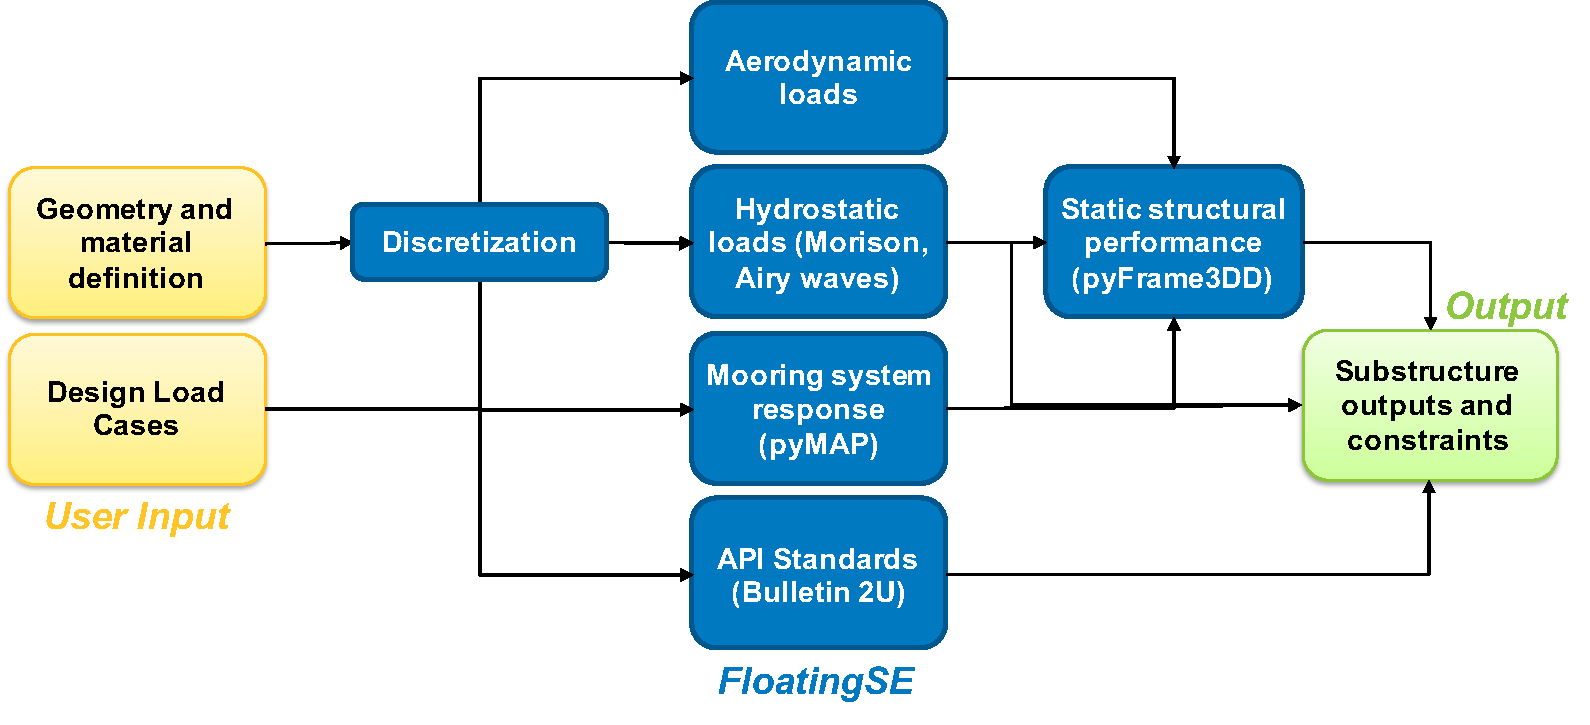
\includegraphics[width=5in]{figs/floatingse}
    \caption{Conceptual diagram of \textit{FloatingSE} execution.}
    \label{fig:floatingse}
  \end{center}
\end{figure}

%\begin{table}
%  \begin{center}
%    \caption{Components and sub-groups within \textit{FloatingSE}.}
%    \label{tbl:exec}
{\small
  \begin{tabularx}{\linewidth}{ l l l X }
    &  \textbf{Prefix} & \textbf{Name} & \textbf{Description} \\
    1) & \texttt{tow} & \textit{TowerLeanSE} & Discretization of tower
    geometry (but no analysis) \\
    2) & \texttt{base} & \textit{Column} & Discretization and API
    Bulletin 2U compliance of base vertical column \\
    3) & \texttt{aux} & \textit{Column} & Discretization and API
    Bulletin 2U compliance of auxiliary columns \\
    4) & \texttt{load} & \textit{FloatingLoading} & Structural analysis
    of comoplete floating turbine load path using \textit{pyFrame3DD} \\
    5) & \texttt{sg} & \textit{SubstructureGeometry} & Geometrical constraints
    on substructure \\
    6) & \texttt{mm} & \textit{MapMooring} & Mooring system analysis using MAP++ program \\
    7) & \texttt{stab} & \textit{SemiStable} & Static stability and final mass and cost summation for generic substructure \\
  \end{tabularx}
}
%\end{center}
%\end{table}

Outputs are accumulated in each sub-group or component,
and they either become inputs to other components, become constraints
for optimization problems, become design variables for optimization
problems, or can simply be ignored.  Currently, a single execution of
FloatingSE takes only a handful of seconds on a modern laptop computer.

In an OpenMDAO group, sub-groups and components are given prefixes in to
aid in referring to specific variables.  These prefixes appear in some
of the variable names listed above (e.g., \texttt{base.waveLoads.mu})
and will appear in the discussion of optimization constraints in Section
\ref{sec:opt}.

\subsection{Examples}
As mentioned in Section \ref{sec:package}, two files are meant as
analysis starting points, \texttt{sparInstance.py} and
\texttt{semiInstance.py}.  These files are encoded with default starting
configurations (from \citet{OC3} and \citet{OC4}, respectively).  They
also have ready configurations for optimization with design variables,
constraints, and solvers options.  However, the flexible and
object-oriented approach to programming these capabilities means that
some complexity was introduced into the code and it becomes more
difficult to use them as simple examples.  For demonstration purposes,
the spar and semisubmersible examples from OC3 and OC4 are also provided
at the bottom of the \texttt{floating.py} file, and are copied below.

TODO PIC ExAMPLES

\subsubsection{Spar}
\begin{lstlisting}
# Number of sections to be used in the design
nsection = 5

# Initialize OpenMDAO problem and FloatingSE Group
prob = Problem(root=FloatingSE(nsection))
prob.setup()

# Remove all auxiliary columns
prob['number_of_auxiliary_columns'] = 0
prob['cross_attachment_pontoons']   = False
prob['lower_attachment_pontoons']   = False
prob['upper_attachment_pontoons']   = False
prob['lower_ring_pontoons']         = False
prob['upper_ring_pontoons']         = False
prob['outer_cross_pontoons']        = False

# Set environment to that used in OC3 testing campaign
prob['water_depth'] = 320.0  # Distance to sea floor [m]
prob['hmax']        = 10.8   # Significant wave height [m]
prob['T']           = 9.8    # Wave period [s]
prob['Uref']        = 11.0   # Wind reference speed [m/s]
prob['zref']        = 119.0  # Wind reference height [m]
prob['shearExp']    = 0.11   # Shear exponent in wind power law
prob['cm']          = 2.0    # Added mass coefficient
prob['Uc']          = 0.0    # Mean current speed
prob['z0']          = 0.0    # Water line
prob['yaw']         = 0.0    # Turbine yaw angle
prob['beta']        = 0.0    # Wind beta angle
prob['cd_usr']      = np.inf # Compute drag coefficient

# Wind and water properties
prob['base.windLoads.rho'] = 1.226   # Density of air [kg/m^3]
prob['base.windLoads.mu']  = 1.78e-5 # Viscosity of air [kg/m/s]
prob['water_density']      = 1025.0  # Density of water [kg/m^3]
prob['base.waveLoads.mu']  = 1.08e-3 # Viscosity of water [kg/m/s]

# Material properties
prob['material_density'] = 7850.0          # Steel [kg/m^3]
prob['E']                = 200e9           # Young's modulus [N/m^2]
prob['G']                = 79.3e9          # Shear modulus [N/m^2]
prob['yield_stress']     = 3.45e8          # Elastic yield stress [N/m^2]
prob['nu']               = 0.26            # Poisson's ratio
prob['permanent_ballast_density'] = 4492.0 # [kg/m^3]

# Mass and cost scaling factors
prob['bulkhead_mass_factor']     = 1.0     # Scaling for unaccounted bulkhead mass
prob['ring_mass_factor']         = 1.0     # Scaling for unaccounted stiffener mass
prob['shell_mass_factor']        = 1.0     # Scaling for unaccounted shell mass
prob['column_mass_factor']       = 1.05    # Scaling for unaccounted column mass
prob['outfitting_mass_fraction'] = 0.06    # Fraction of additional outfitting mass for each column
prob['ballast_cost_rate']        = 100.0   # Cost factor for ballast mass [USD/kg]
prob['tapered_col_cost_rate']    = 4720.0  # Cost factor for column mass [USD/kg]
prob['outfitting_cost_rate']     = 6980.0  # Cost factor for outfitting mass [USD/kg]
prob['mooring_cost_rate']        = 1.1     # Cost factor for mooring mass [USD/kg]

TODO: DON'T NEED THESE?

# Safety factors
prob['gamma_f'] = 1.35 # Safety factor on loads
prob['gamma_b'] = 1.1  # Safety factor on buckling
prob['gamma_m'] = 1.1  # Safety factor on materials
prob['gamma_n'] = 1.0  # Safety factor on consequence of failure
prob['gamma_fatigue'] = 1.755 # Not used

# Column geometry
prob['base_permanent_ballast_height'] = 10.0 # Height above keel for permanent ballast [m]
prob['base_freeboard']                = 10.0 # Height extension above waterline [m]
prob['base_section_height'] = np.array([36.0, 36.0, 36.0, 8.0, 14.0])  # Length of each section [m]
prob['base_outer_diameter'] = np.array([9.4, 9.4, 9.4, 9.4, 6.5, 6.5]) # Diameter at each section node (linear lofting between) [m]
prob['base_wall_thickness'] = 0.05 * np.ones(nsection+1)               # Shell thickness at each section node (linear lofting between) [m]
prob['base_bulkhead_nodes'] = [True, True, False, False, False, False] # Locations of internal bulkheads at section interfaces

# Column ring stiffener parameters
prob['base_stiffener_web_height']       = 0.10 * np.ones(nsection) # (by section) [m]
prob['base_stiffener_web_thickness']    = 0.04 * np.ones(nsection) # (by section) [m]
prob['base_stiffener_flange_width']     = 0.10 * np.ones(nsection) # (by section) [m]
prob['base_stiffener_flange_thickness'] = 0.02 * np.ones(nsection) # (by section) [m]
prob['base_stiffener_spacing']          = 0.40 * np.ones(nsection) # (by section) [m]

# Mooring parameters
prob['number_of_mooring_lines']    = 3             # Evenly spaced around structure
prob['mooring_type']               = 'chain'       # Options are chain, nylon, polyester, fiber, or iwrc
prob['anchor_type']                = 'suctionpile' # Options are SUCTIONPILE or DRAGEMBEDMENT
prob['mooring_diameter']           = 0.09          # Diameter of mooring line/chain [m]
prob['fairlead']                   = 70.0          # Distance below waterline for attachment [m]
prob['fairlead_offset_from_shell'] = 0.5           # Offset from shell surface for mooring attachment [m]
prob['scope_ratio']                = 3.6088        # Ratio of line length to distance to sea floor (from fairlead)
prob['anchor_radius']              = 853.87        # Distance from centerline to sea floor landing [m]
prob['drag_embedment_extra_length'] = 300.0        # Extra length beyond sea flor landing to ensure anchors only see horizontal forces [m]

# Porperties of turbine tower
prob['hub_height']              = 87.6                              # Length from tower base to top (not including freeboard) [m]
prob['tower_section_height']    = 87.6/nsection * np.ones(nsection) # Length of each tower section [m]
prob['tower_outer_diameter']    = 6.50 * np.ones(nsection+1)        # Diameter at each tower section node (linear lofting between) [m]
prob['tower_wall_thickness']    = 0.05 * np.ones(nsection+1)        # Diameter at each tower section node (linear lofting between) [m]
prob['tower_buckling_length']   = 30.0                              # Tower buckling reinforcement spacing [m]
prob['tower_outfitting_factor'] = 1.07                              # Scaling for unaccounted tower mass in outfitting

# Properties of rotor-nacelle-assembly (RNA)
prob['rna_mass']   = 285598.8 # Mass [kg]
prob['rna_I']      = 1e5*np.array([1149.307, 220.354, 187.597, 0, 5.037, 0]) # Moment of intertia (xx,yy,zz,xy,xz,yz) [kg/m^2]
prob['rna_cg']     = np.array([-1.132, 0, 0.509])                       # Offset of RNA center of mass from tower top (x,y,z) [m]
prob['rna_force']  = np.array([1284744.196, 0, -2914124.844])           # Net force acting on RNA (x,y,z) [N]
prob['rna_moment'] = np.array([3963732.762, -2275104.794, -346781.682]) # Net moment acting on RNA (x,y,z) [N*m]

# Execute FloatingSE
prob.run()

\end{lstlisting}

\subsubsection{Semisubmersible}
\begin{lstlisting}
# Number of sections to be used in the design
nsection = 5

# Initialize OpenMDAO problem and FloatingSE Group
prob = Problem(root=FloatingSE(nsection))
prob.setup()

# Add in auxiliary columns and truss elements
prob['number_of_auxiliary_columns'] = 3
prob['cross_attachment_pontoons']   = True # Lower-Upper base-to-auxiliary connecting cross braces
prob['lower_attachment_pontoons']   = True # Lower base-to-auxiliary connecting pontoons
prob['upper_attachment_pontoons']   = True # Upper base-to-auxiliary connecting pontoons
prob['lower_ring_pontoons']         = True # Lower ring of pontoons connecting auxiliary columns
prob['upper_ring_pontoons']         = True # Upper ring of pontoons connecting auxiliary columns
prob['outer_cross_pontoons']        = True # Auxiliary ring connecting V-cross braces

# Set environment to that used in OC4 testing campaign
prob['water_depth'] = 200.0  # Distance to sea floor [m]
prob['hmax']        = 10.8   # Significant wave height [m]
prob['T']           = 9.8    # Wave period [s]
prob['Uref']        = 11.0   # Wind reference speed [m/s]
prob['zref']        = 119.0  # Wind reference height [m]
prob['shearExp']    = 0.11   # Shear exponent in wind power law
prob['cm']          = 2.0    # Added mass coefficient
prob['Uc']          = 0.0    # Mean current speed
prob['z0']          = 0.0    # Water line
prob['yaw']         = 0.0    # Turbine yaw angle
prob['beta']        = 0.0    # Wind beta angle
prob['cd_usr']      = np.inf # Compute drag coefficient

# Wind and water properties
prob['base.windLoads.rho'] = 1.226   # Density of air [kg/m^3]
prob['base.windLoads.mu']  = 1.78e-5 # Viscosity of air [kg/m/s]
prob['water_density']      = 1025.0  # Density of water [kg/m^3]
prob['base.waveLoads.mu']  = 1.08e-3 # Viscosity of water [kg/m/s]

# Material properties
prob['material_density'] = 7850.0          # Steel [kg/m^3]
prob['E']                = 200e9           # Young's modulus [N/m^2]
prob['G']                = 79.3e9          # Shear modulus [N/m^2]
prob['yield_stress']     = 3.45e8          # Elastic yield stress [N/m^2]
prob['nu']               = 0.26            # Poisson's ratio
prob['permanent_ballast_density'] = 4492.0 # [kg/m^3]

# Mass and cost scaling factors
prob['bulkhead_mass_factor']     = 1.0     # Scaling for unaccounted bulkhead mass
prob['ring_mass_factor']         = 1.0     # Scaling for unaccounted stiffener mass
prob['shell_mass_factor']        = 1.0     # Scaling for unaccounted shell mass
prob['column_mass_factor']       = 1.05    # Scaling for unaccounted column mass
prob['outfitting_mass_fraction'] = 0.06    # Fraction of additional outfitting mass for each column
prob['ballast_cost_rate']        = 100.0   # Cost factor for ballast mass [USD/kg]
prob['tapered_col_cost_rate']    = 4720.0  # Cost factor for column mass [USD/kg]
prob['outfitting_cost_rate']     = 6980.0  # Cost factor for outfitting mass [USD/kg]
prob['mooring_cost_rate']        = 1.1     # Cost factor for mooring mass [USD/kg]
prob['pontoon_cost_rate']        = 6.250   # Cost factor for pontoons [USD/kg]

# Safety factors
prob['gamma_f'] = 1.35 # Safety factor on loads
prob['gamma_b'] = 1.1  # Safety factor on buckling
prob['gamma_m'] = 1.1  # Safety factor on materials
prob['gamma_n'] = 1.0  # Safety factor on consequence of failure
prob['gamma_fatigue'] = 1.755 # Not used

# Column geometry
prob['base_permanent_ballast_height'] = 10.0 # Height above keel for permanent ballast [m]
prob['base_freeboard']                = 10.0 # Height extension above waterline [m]
prob['base_section_height'] = np.array([36.0, 36.0, 36.0, 8.0, 14.0])  # Length of each section [m]
prob['base_outer_diameter'] = np.array([9.4, 9.4, 9.4, 9.4, 6.5, 6.5]) # Diameter at each section node (linear lofting between) [m]
prob['base_wall_thickness'] = 0.05 * np.ones(nsection+1)               # Shell thickness at each section node (linear lofting between) [m]
prob['base_bulkhead_nodes'] = [True, True, False, False, False, False] # Locations of internal bulkheads at section interfaces

# Auxiliary column geometry
prob['radius_to_auxiliary_column']         = 33.333 * np.cos(np.pi/6) # Centerline of base column to centerline of auxiliary column [m]
prob['auxiliary_permanent_ballast_height'] = 0.1                      # Height above keel for permanent ballast [m]
prob['auxiliary_freeboard']                = 12.0                     # Height extension above waterline [m]
prob['auxiliary_section_height']           = np.array([6.0, 0.1, 7.9, 8.0, 10]) # Length of each section [m]
prob['auxiliary_outer_diameter']           = np.array([24, 24, 12, 12, 12, 12]) # Diameter at each section node (linear lofting between) [m]
prob['auxiliary_wall_thickness']           = 0.06 * np.ones(nsection+1)         # Shell thickness at each section node (linear lofting between) [m]

# Column ring stiffener parameters
prob['base_stiffener_web_height']       = 0.10 * np.ones(nsection) # (by section) [m]
prob['base_stiffener_web_thickness']    = 0.04 * np.ones(nsection) # (by section) [m]
prob['base_stiffener_flange_width']     = 0.10 * np.ones(nsection) # (by section) [m]
prob['base_stiffener_flange_thickness'] = 0.02 * np.ones(nsection) # (by section) [m]
prob['base_stiffener_spacing']          = 0.40 * np.ones(nsection) # (by section) [m]

# Auxiliary column ring stiffener parameters
prob['auxiliary_stiffener_web_height']       = 0.10 * np.ones(nsection) # (by section) [m]
prob['auxiliary_stiffener_web_thickness']    = 0.04 * np.ones(nsection) # (by section) [m]
prob['auxiliary_stiffener_flange_width']     = 0.01 * np.ones(nsection) # (by section) [m]
prob['auxiliary_stiffener_flange_thickness'] = 0.02 * np.ones(nsection) # (by section) [m]
prob['auxiliary_stiffener_spacing']          = 0.40 * np.ones(nsection) # (by section) [m]

# Pontoon parameters
prob['pontoon_outer_diameter']    = 3.2    # Diameter of all pontoon/truss elements [m]
prob['pontoon_wall_thickness']    = 0.0175 # Thickness of all pontoon/truss elements [m]
prob['base_pontoon_attach_lower'] = -20.0  # Lower z-coordinate on base where truss attaches [m]
prob['base_pontoon_attach_upper'] = 10.0   # Upper z-coordinate on base where truss attaches [m]

# Mooring parameters
prob['number_of_mooring_lines']    = 3             # Evenly spaced around structure
prob['mooring_type']               = 'chain'       # Options are chain, nylon, polyester, fiber, or iwrc
prob['anchor_type']                = 'suctionpile' # Options are SUCTIONPILE or DRAGEMBEDMENT
prob['mooring_diameter']           = 0.0766        # Diameter of mooring line/chain [m]
prob['fairlead']                   = 14.0          # Distance below waterline for attachment [m]
prob['fairlead_offset_from_shell'] = 0.5           # Offset from shell surface for mooring attachment [m]
prob['scope_ratio']                = 4.4919        # Ratio of line length to distance to sea floor (from fairlead)
prob['anchor_radius']              = 837.6         # Distance from centerline to sea floor landing [m]
prob['drag_embedment_extra_length'] = 300.0        # Extra length beyond sea flor landing to ensure anchors only see horizontal forces [m]

# Porperties of turbine tower
prob['hub_height']              = 87.6                              # Length from tower base to top (not including freeboard) [m]
prob['tower_section_height']    = 87.6/nsection * np.ones(nsection) # Length of each tower section [m]
prob['tower_outer_diameter']    = 6.50 * np.ones(nsection+1)        # Diameter at each tower section node (linear lofting between) [m]
prob['tower_wall_thickness']    = 0.05 * np.ones(nsection+1)        # Diameter at each tower section node (linear lofting between) [m]
prob['tower_buckling_length']   = 30.0                              # Tower buckling reinforcement spacing [m]
prob['tower_outfitting_factor'] = 1.07                              # Scaling for unaccounted tower mass in outfitting

# Properties of rotor-nacelle-assembly (RNA)
prob['rna_mass']   = 285598.8 # Mass [kg]
prob['rna_I']      = 1e5*np.array([1149.307, 220.354, 187.597, 0, 5.037, 0]) # Moment of intertia (xx,yy,zz,xy,xz,yz) [kg/m^2]
prob['rna_cg']     = np.array([-1.132, 0, 0.509])                       # Offset of RNA center of mass from tower top (x,y,z) [m]
prob['rna_force']  = np.array([1284744.196, 0, -2914124.844])           # Net force acting on RNA (x,y,z) [N]
prob['rna_moment'] = np.array([3963732.762, -2275104.794, -346781.682]) # Net moment acting on RNA (x,y,z) [N*m]

# Execute FloatingSE
prob.run()
\end{lstlisting}
